Soit $k$ un réel strictement positif. Le but de cet exercice est de déterminer le nombre de solutions de l'équation $\ln(x)=kx$ de paramètre $k$.

\medskip

\begin{enumerate}
	\item \underline{Conjectures graphiques :}
	
	\smallskip
	
	On a représenté, ci-dessous, dans un repère orthogonal, la courbe d'équation $y = \ln(x)$, la droite d'équation $y = x$ ainsi que la droite d'équation $y=0,2x$ :
	%
	\begin{center}
		\begin{tikzpicture}[x=0.75cm,y=0.75cm,xmin=-1,xmax=17,xgrille=1,xgrilles=0.5,ymin=-2,ymax=9,ygrille=1,ygrilles=0.5]
			\GrilleTikz[Affs=false]
			\AxesTikz[ElargirOx=0/0,ElargirOy=0/0] \AxexTikz{1,2,...,16} \AxeyTikz[AffOrigine=false]{-2,-1,...,8}
			\OrigineTikz
			\clip (\xmin,\ymin) rectangle (\xmax,\ymax) ;
			\draw[very thick,red,samples=250,domain=0.1:\xmax] plot (\x,{ln(\x)}) ;
			\draw[red] (9,3) node[font=\Large] {$y=\ln(x)$} ;
			\draw[thick,blue,samples=2,domain=0:\xmax] plot (\x,\x) ;
			\draw[blue] (5,6.5) node[font=\Large] {$y=x$} ;
			\draw[thick,CouleurVertForet,samples=2,domain=0:\xmax] plot (\x,{0.2*\x}) ;
			\draw[CouleurVertForet] (5.5,0.5) node[font=\Large] {$y=0,2x$} ;
		\end{tikzpicture}
	\end{center}
	%
	À partir du graphique ci-dessus, conjecturer le nombre de solutions de l'équation $\ln(x)=kx$ pour $k = 1$ puis pour $k = 0,2$.
	
	\vspace{2.5mm}
	\item \underline{Étude du cas $k = 1$ :}
	
	\smallskip
	
	On considère la fonction $f$, définie et dérivable sur $]0;+\infty[$, par : $f(x) = \ln(x)-x$.
	
	On note $f'$ la fonction dérivée de la fonction $f$.
	\begin{enumerate}
		\item Calculer $f'(x)$.
		\item Étudier le sens de variation de la fonction $f$ sur $]0;+\infty[$.
		
		Dresser le tableau des variations de la fonction $f$ en y faisant figurer la valeur exacte des extrema s'il y en a. Les limites aux bornes de l'intervalle de définition ne sont pas attendues. 
		\item En déduire le nombre de solutions de l'équation $\ln(x)=x$.
		
		\vspace{2.5mm}
	\end{enumerate}
	\item \underline{Étude du cas général :}
	
	\smallskip
	
	$k$ est un nombre réel strictement positif. On considère la fonction $g$ définie sur $]0;+\infty[$ par :
	
	$g(x)=\ln(x)-kx$.
	
	\smallskip
	
	On admet que le tableau des variations de la fonction $g$ est le suivant :
	
	\begin{center}
		\begin{tikzpicture}[double distance=2pt]
			\tkzTabInit{$x$/1,$g(x)$/2}{$0$,$\frac{1}{k}$,$+\infty$}
			\tkzTabVar{D-/$-\infty$,+/$g\left(\frac{1}{k}\right)$,-/$-\infty$}
		\end{tikzpicture}
	\end{center}
	\begin{enumerate}
		\item Donner, en fonction du signe de $g\left(\frac{1}{k}\right)$, le nombre de solutions de l'équation $g(x)= 0$.
		\item Calculer $g\left(\frac{1}{k}\right)$ en fonction du réel $k$
		\item Monter que $g\left(\frac{1}{k}\right) > 0$ équivaut à $\ln(k) < -1$.
		\item Déterminer l'ensemble des valeurs de $k$ pour lesquelles l'équation $\ln(x)=kx$ possède exactement deux solutions.
		\item Donner, selon les valeurs de $k$, le nombre de solutions de l'équation $\ln(x)=kx$.
	\end{enumerate}
\end{enumerate}